\documentclass[10pt]{beamer}


\usetheme{metropolis}
\usepackage{appendixnumberbeamer}


\usepackage{booktabs}
\usepackage[scale=2]{ccicons}

\usepackage{pgfplots}
\usepgfplotslibrary{dateplot}

\usepackage{xspace}
\newcommand{\themename}{\textbf{\textsc{metropolis}}\xspace}


\usepackage{graphicx} % http://ctan.org/pkg/graphicx (don't use 'demo' in your document)
\usepackage{xcolor}
\usepackage{adjustbox}

\usepackage[utf8]{inputenc}

% REMOVE PAGE NUMERING:
\setbeamertemplate{footline}[frame number]{} % gets rid of bottom navigation bars
\setbeamertemplate{navigation symbols}{}  % gets rid of bottom navigation symbols
\setbeamertemplate{footline}{}  % gets rid of footer
%will override 'frame number' instruction above
%comment out to revert to previous/default definitions	

\title{Vorhersage und Interpretation des\\Verkaufpreises von Immobilien\\mittels linearer Regression}
\date{}
\author{Karin Lassnig, Phillip Grafendorfer, Martin Huf, Raphael Peer}



\begin{document}

\setbeamerfont{frametitle}{size=\Large}
\setbeamertemplate{frametitle}[default][center]

\maketitle

\section{Daten}


\begin{frame}{Ames House price Dataset}
	
	Datensatz...
	
	\begin{tiny}		
		Quelle:\\
		\url{https://www.kaggle.com/c/house-prices-advanced-regression-techniques}
	\end{tiny}
\end{frame}


\begin{frame}{Fehlende Werte: Übersicht}
	
	\begin{figure}
		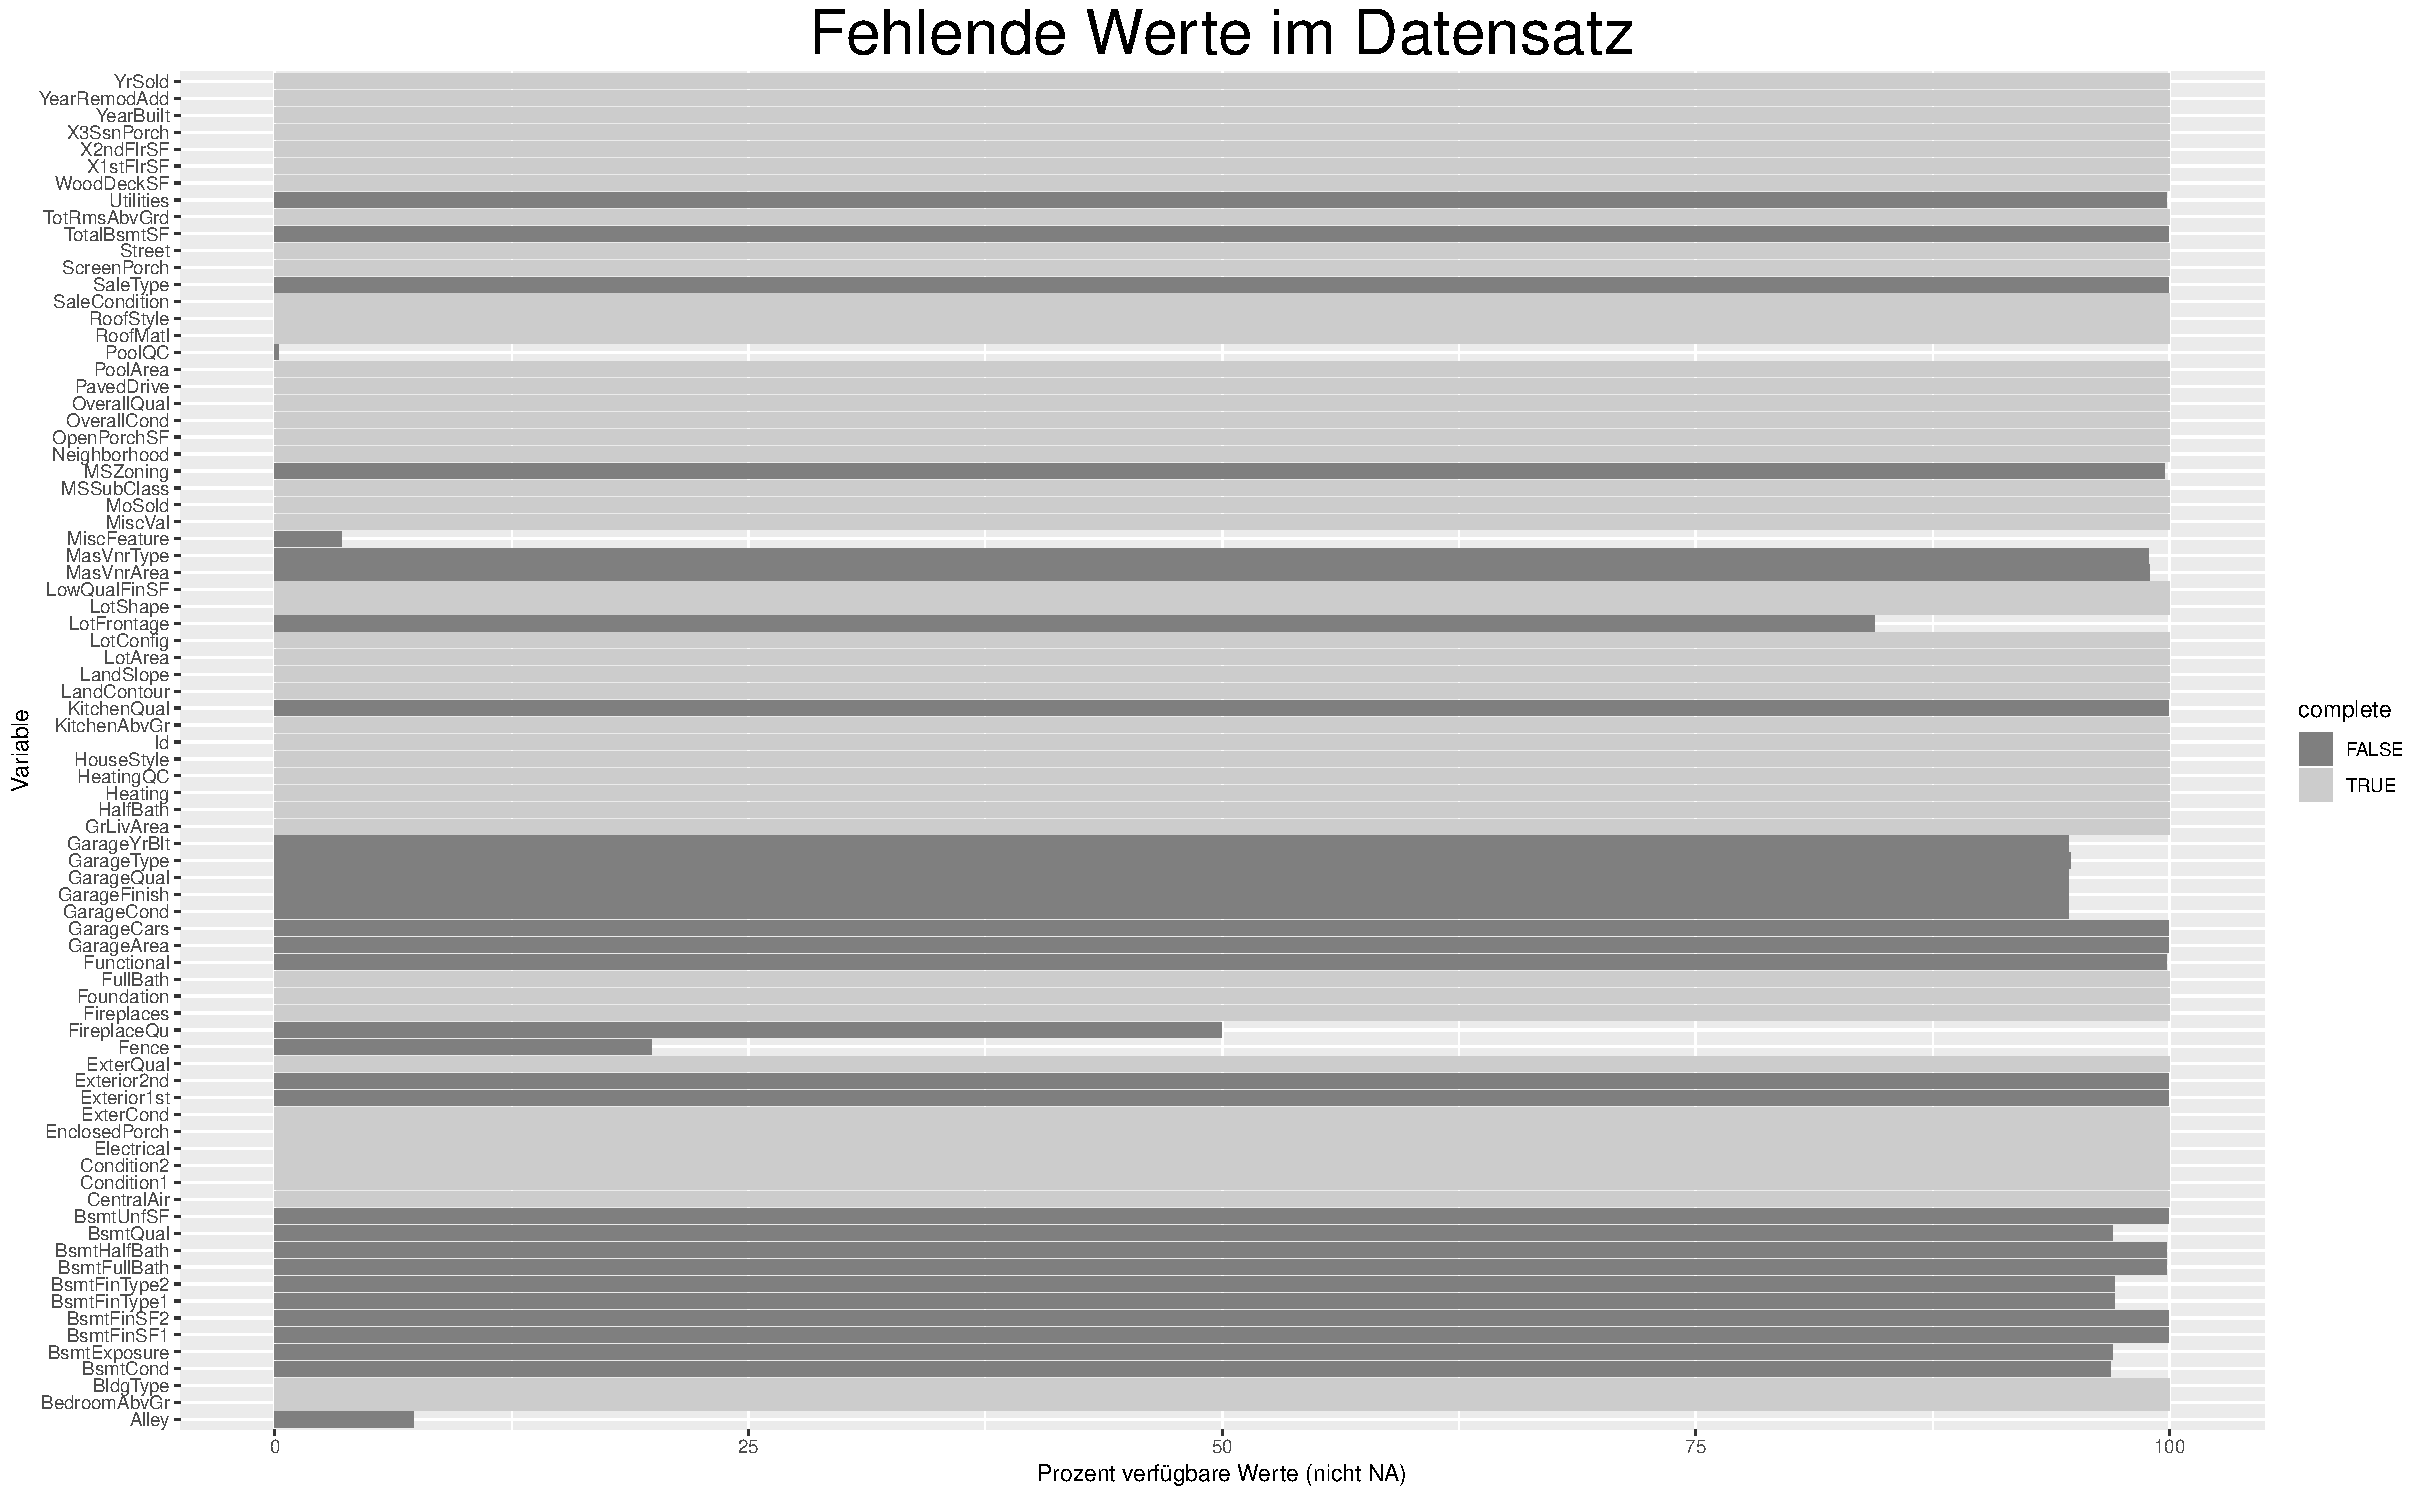
\includegraphics[width=\textwidth, keepaspectratio]{figures/na_stats}
	\end{figure}
	
\end{frame}

\begin{frame}{Fehlende Werte: Strategie}
	
	\begin{Large}{Umgang mit fehlenden Werten:}\end{Large}
	\begin{itemize}
		\item Bei mehr als 10\% Fehlenden Werten: Variable verworfen
		\item Bei numerischen Variablen: NA durch Median der Variable ersetzt
		\item Bei kategorischen Variablen: NA als eigene Kategorie (Kategorie 'unbekannt')
	\end{itemize}
	
\end{frame}


\begin{frame}{...}
	

\end{frame}


\section{Modelle}

\begin{frame}{Einfaches Model}
	
	\begin{Large}{Eckdaten}\end{Large}
	\begin{itemize}
		\item 73 erklärende Variablen
		\item keine manuelle Auswahl der Variablen
		\item Mean absolute deviation: $\approx 15 000 \$$
	\end{itemize}
	
\end{frame}

\begin{frame}{Einfaches Model}
	
	\begin{figure}
		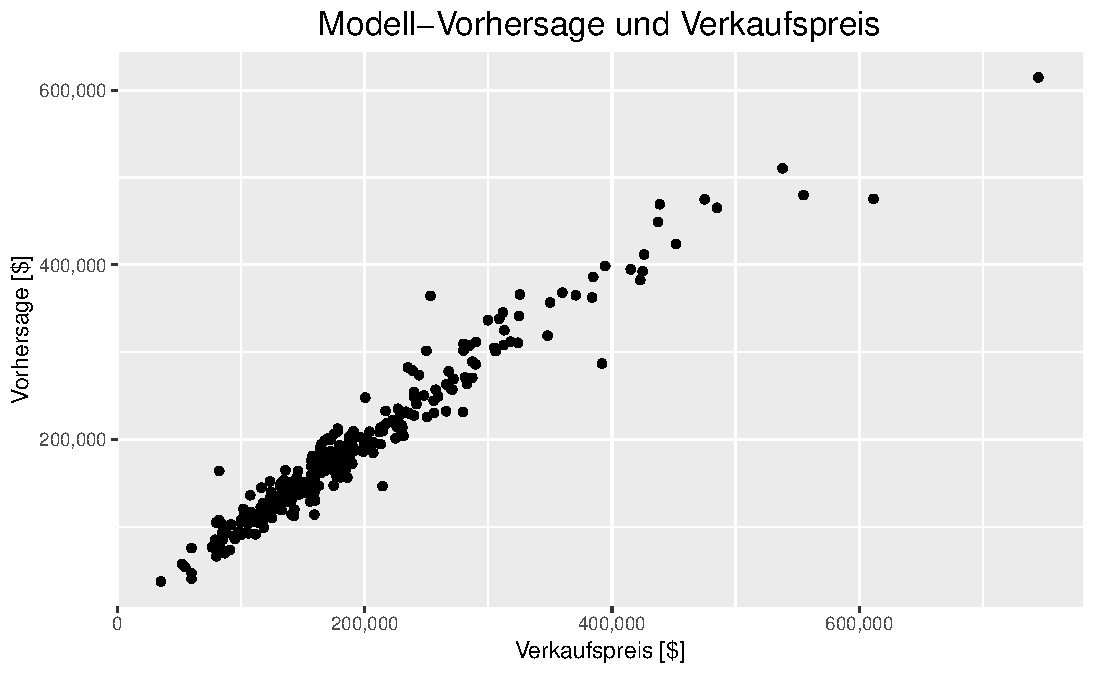
\includegraphics[width=\textwidth, keepaspectratio]{figures/simple_model}
	\end{figure}
	
\end{frame}

\section{Standardisierte Koeffizienten}

\begin{frame}{Problemstellung}
	
	\begin{Large}{Nachteil unstandardisierter Regressionskoeffizienten}\end{Large}
	
	  \begin{itemize}
		\item Von den Maßeinheiten für X und Y abhängig
		\item Daher schlechtere Vergleichbarkeit
	  \end{itemize}
	 
	\begin{Large}{Lösung: Standardisierte Koeffizienten}\end{Large}
	  
	
\end{frame}


\begin{frame}{Umsetzung}
	
	\begin{Large}{Abhängige und unabhängige Variablen werden standardisiert}\end{Large}
	
	\begin{itemize}
		\item Mittelwert = 0
		\item Varianz = 1
	\end{itemize}
	
	\begin{Large}{Regressionskoeffizienten:}\end{Large}
		\begin{itemize}
     	       \item $\hat{\beta_i} = \beta_i*\frac{s_{x_i}}{s_y}$
     	       \item $\hat{\beta_i}$ sollte im Intervall [-1, 1] liegen (sonst Hinweis auf Multikollinearität )
		\end{itemize}
	
\end{frame}



\begin{frame}{Vor- und Nachteile}
	
	\begin{Large}{Vorteile}\end{Large}
	
	\begin{itemize}
		\item Operiert mit Änderungen von Standardabweichungen
		\item $\Rightarrow$ Stärke und Richtung eines Effektes können besser interpretiert und verglichen werden
	\end{itemize}
	
	\begin{Large}{Nachteile}\end{Large}
	
	  \begin{itemize}
		\item Nur für Variablen anwendbar, bei denen Heranziehen einer Standardabweichung sinnvoll ist (zB nicht Dummyvariablen)
		\item Abhängigkeit von Stichprobe
		\item Kann zu Missverständnissen führen
	  \end{itemize}
	
\end{frame}

\begin{frame}{Anwendung}
	
	\begin{figure}
		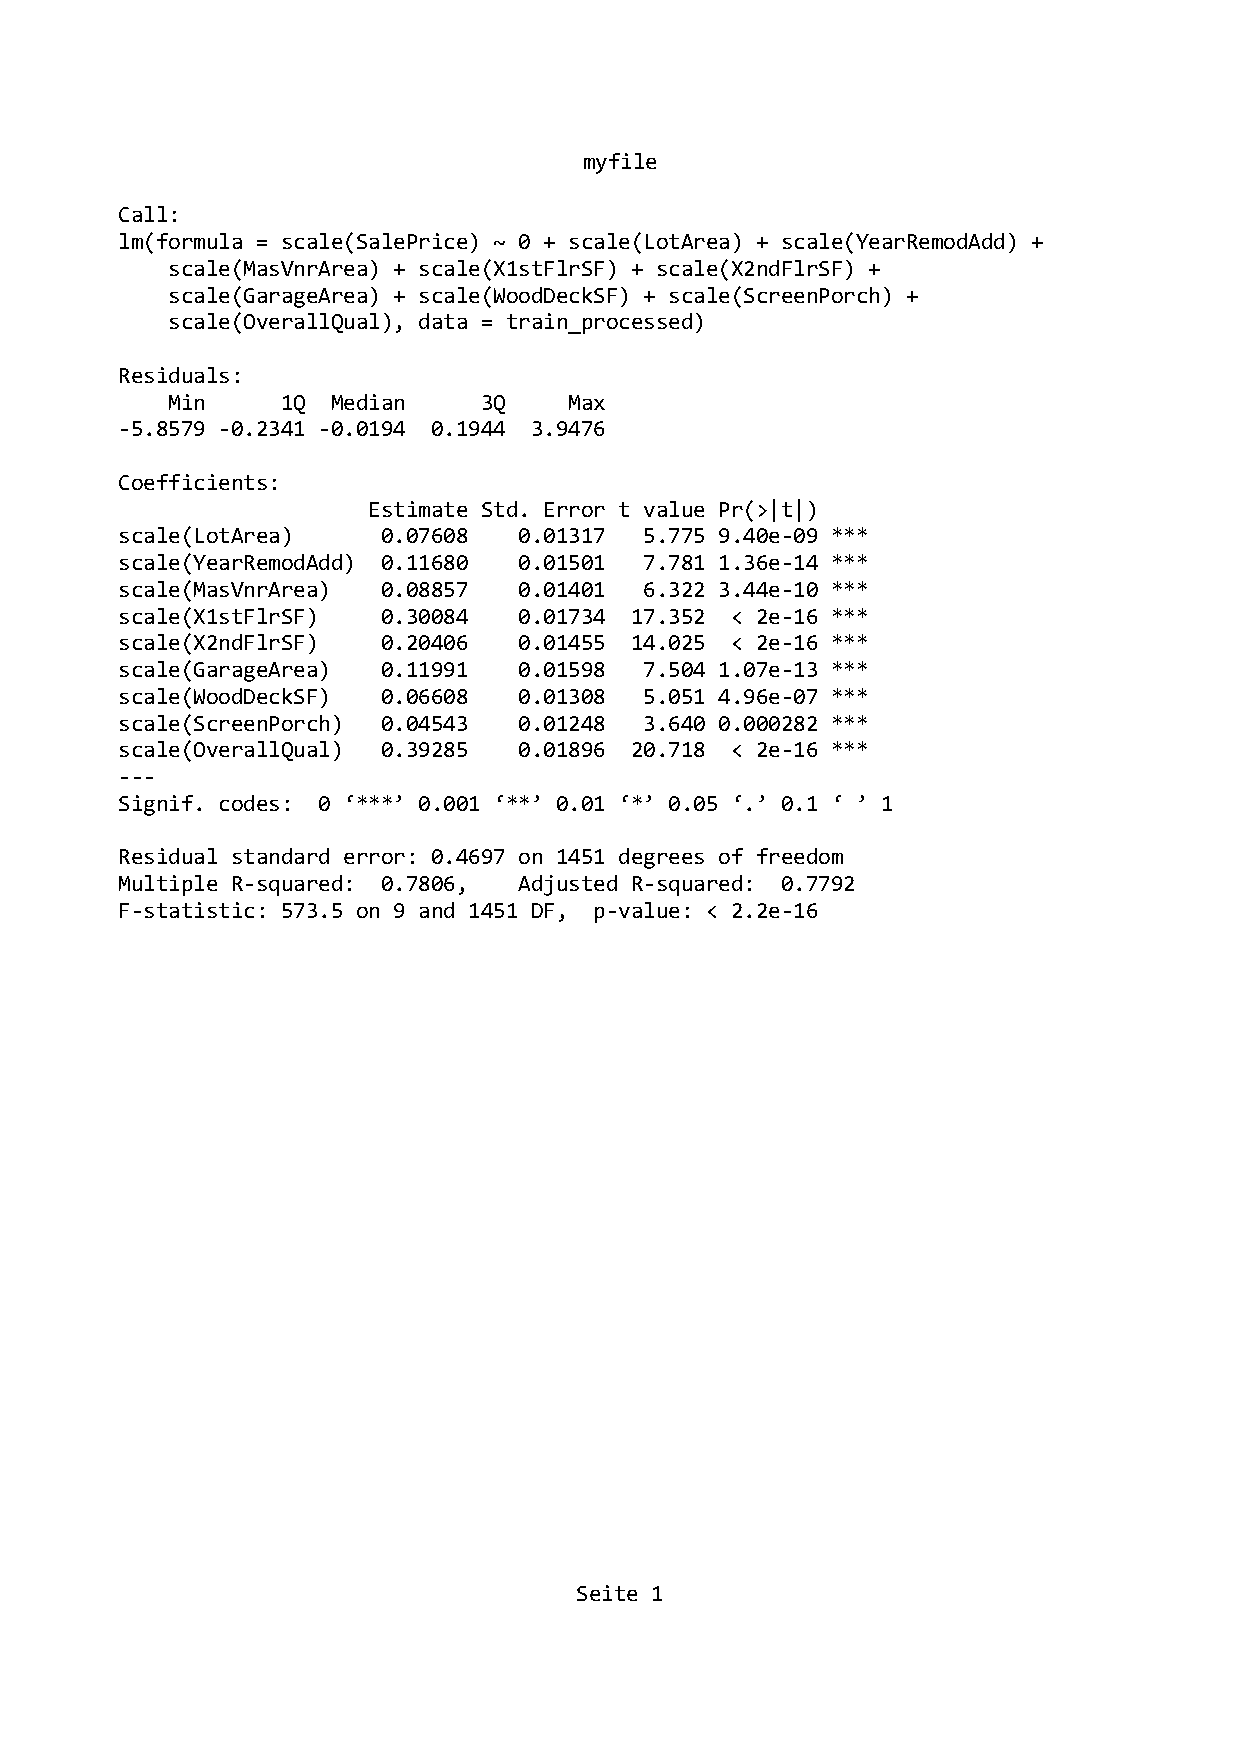
\includegraphics[width=\textwidth, keepaspectratio]{figures/Stand_M}
	\end{figure}

	
\end{frame}	

\begin{frame}{Fragen und Diskussion}
	\begin{LARGE}
		\begin{center}
			Vielen Dank für Ihre Aufmerksamkeit
		\end{center}
	\end{LARGE}
\end{frame}

\end{document}
